%%%%%%%%%%%%%%%%%%%%%%%%%%%%%%%%%%%%%%%%%%%%%%%%%%%%%%%%%%%%%%%%%%%%%
%% This is a "template" model document for submission to the
%% American Chemical Society (ACS).
%%
%% The guidance here contains information about how you may wish to
%% modify it to match the requirements of various ACS journals. The
%% ACS do *not* typeset accepted articles using LaTeX, so there is
%% no specific class required.
%%
%% This template deliberately does *not* seek to reproduce
%% the layout of the typeset journal: this is explicitly not
%% required by the ACS for LaTeX submissions.
%%
%% Please report any issues with the template at
%% https://github.com/josephwright/acs-template/issues
%%
%% Released under the Creative Commons 0 license
%% https://creativecommons.org/public-domain/cc0/
%% 
%% Copyight (c) 2025 Joseph Wright
%%%%%%%%%%%%%%%%%%%%%%%%%%%%%%%%%%%%%%%%%%%%%%%%%%%%%%%%%%%%%%%%%%%%%
\documentclass[letterpaper]{article}

%%%%%%%%%%%%%%%%%%%%%%%%%%%%%%%%%%%%%%%%%%%%%%%%%%%%%%%%%%%%%%%%%%%%%
%% Font setup - delete if you are using LuaLaTeX
%%%%%%%%%%%%%%%%%%%%%%%%%%%%%%%%%%%%%%%%%%%%%%%%%%%%%%%%%%%%%%%%%%%%%
\usepackage[T1]{fontenc}

%%%%%%%%%%%%%%%%%%%%%%%%%%%%%%%%%%%%%%%%%%%%%%%%%%%%%%%%%%%%%%%%%%%%%
%% Adjust the margins and allow for line spacing
%%%%%%%%%%%%%%%%%%%%%%%%%%%%%%%%%%%%%%%%%%%%%%%%%%%%%%%%%%%%%%%%%%%%%
\usepackage{geometry}
\geometry{margin = 1in}
\usepackage{setspace}

%%%%%%%%%%%%%%%%%%%%%%%%%%%%%%%%%%%%%%%%%%%%%%%%%%%%%%%%%%%%%%%%%%%%%
%% Reference support
%%
%% The recommended method for producing the reference section is
%% to use biblatex. If you wish to use a classical BibTeX
%% approach, this is easiest to achieve using the achemso package.
%% In that case, you should remove the biblatex lines.
%%%%%%%%%%%%%%%%%%%%%%%%%%%%%%%%%%%%%%%%%%%%%%%%%%%%%%%%%%%%%%%%%%%%%
% You can adjust the printing of DOI, article title, etc. using
% package options, e.g. "doi = true"; see the biblatex manual for
% details of adjusting the number of authors printed, e.g.
% "maxnames = 15" to print no more than 15 authors.
\usepackage[style = chem-acs]{biblatex}
\addbibresource{references.bib}
% If you are using classical BibTeX, remove the above lines and 
% uncomment:
%\usepackage{achemso}

%%%%%%%%%%%%%%%%%%%%%%%%%%%%%%%%%%%%%%%%%%%%%%%%%%%%%%%%%%%%%%%%%%%%%
%% Graphic inclusion and scheme and chart support
%%%%%%%%%%%%%%%%%%%%%%%%%%%%%%%%%%%%%%%%%%%%%%%%%%%%%%%%%%%%%%%%%%%%%
\usepackage{graphicx}
\usepackage{float}
% 补充表跨页排版及历史稿 Unicode 字符兼容；均使用现有 TeX Live 宏包。
\usepackage{array,longtable,booktabs,newunicodechar}
\newunicodechar{–}{\textendash}
\newunicodechar{—}{\textemdash}
\newunicodechar{‐}{-}
\newunicodechar{ń}{\'{n}}
\newunicodechar{μ}{\ensuremath{\mu}}
\newunicodechar{γ}{\ensuremath{\gamma}}
\newunicodechar{δ}{\ensuremath{\delta}}
\newunicodechar{α}{\ensuremath{\alpha}}

%% --- pgfplots/ACS plot styles, ported from legacy preamble ---
\usepackage{xcolor}
\usepackage{pgfplots}
\pgfplotsset{compat = 1.18}
\definecolor{acsblue}{RGB}{72,116,176}
\definecolor{acsred}{RGB}{196,78,82}
\definecolor{acsorange}{RGB}{221,132,82}
\definecolor{acsgray}{RGB}{88,89,91}
\definecolor{acsplotbg}{RGB}{239,241,247}
\pgfplotsset{
  acs axis/.style={
    axis background/.style={fill=acsplotbg},
    axis line style={draw=acsgray, line width=0.45pt},
    tick style={draw=acsgray, line width=0.4pt},
    tick label style={font=\footnotesize},
    label style={font=\small},
    title style={font=\small\bfseries},
    grid=both,
    major grid style={draw=white, line width=0.55pt},
    minor grid style={draw=white, line width=0.3pt},
    minor tick num=1,
    scaled ticks=false,
    legend style={draw=none, fill=none, font=\footnotesize},
    every axis plot/.append style={line width=0.85pt}
  },
  acs xbar/.style={
    acs axis,
    xbar,
    xmin=0,
    width=0.88\linewidth,
    height=6.1cm,
    bar width=8pt,
    enlarge y limits=0.16,
    nodes near coords,
    nodes near coords align={horizontal},
    nodes near coords style={font=\scriptsize, xshift=1.2pt}
  },
  acs ybar/.style={
    acs axis,
    ybar,
    width=0.92\linewidth,
    height=6.1cm,
    bar width=11pt,
    enlarge x limits=0.08,
    nodes near coords,
    nodes near coords align={vertical},
    nodes near coords style={font=\scriptsize, yshift=1pt}
  }
}
%% --- End of pgfplots/ACS plot styles block ---
\newfloat{scheme}{htbp}{los}
\floatname{scheme}{Scheme}
\floatname{chart}{Chart}
\newfloat{graph}{htbp}{loh}

%%%%%%%%%%%%%%%%%%%%%%%%%%%%%%%%%%%%%%%%%%%%%%%%%%%%%%%%%%%%%%%%%%%%%
%% Common support packages
%%%%%%%%%%%%%%%%%%%%%%%%%%%%%%%%%%%%%%%%%%%%%%%%%%%%%%%%%%%%%%%%%%%%%
\usepackage{chemformula} % Formulas using \ch{}
% or
%\usepackage[version = 4]{mhchem} % Formulas using \ce{}

%%%%%%%%%%%%%%%%%%%%%%%%%%%%%%%%%%%%%%%%%%%%%%%%%%%%%%%%%%%%%%%%%%%%%
%% Many journals require that sections are unnumbered: this 
%% is activated here
%%%%%%%%%%%%%%%%%%%%%%%%%%%%%%%%%%%%%%%%%%%%%%%%%%%%%%%%%%%%%%%%%%%%%
\setcounter{secnumdepth}{-1}

%%%%%%%%%%%%%%%%%%%%%%%%%%%%%%%%%%%%%%%%%%%%%%%%%%%%%%%%%%%%%%%%%%%%%
%% Place any additional macros here.  Please use \newcommand* where
%% possible, and avoid layout-changing macros (which are not used
%% when typesetting).
%%%%%%%%%%%%%%%%%%%%%%%%%%%%%%%%%%%%%%%%%%%%%%%%%%%%%%%%%%%%%%%%%%%%%
\newcommand*\mycommand[1]{\texttt{\emph{#1}}}

%%%%%%%%%%%%%%%%%%%%%%%%%%%%%%%%%%%%%%%%%%%%%%%%%%%%%%%%%%%%%%%%%%%%%
%% Author and title data:
%% the authblk package is currently the simplest way to provide this
%%%%%%%%%%%%%%%%%%%%%%%%%%%%%%%%%%%%%%%%%%%%%%%%%%%%%%%%%%%%%%%%%%%%%
\usepackage{authblk}
\author[1]{Xinge Xia}
\author[1]{Fan Wu}
\affil[1]{College of Cyber Security, Jinan University, Guangzhou, China}
\author[2]{Xianyou Duan}
\affil[2]{College of Chemistry and Materials Science, Jinan University, Guangzhou, China}
\author[1]{Hongyi Chen}
\author[1]{Bingwen Feng*}

\title{Selenium Nanoparticle Cytotoxicity Prediction: A Comparative Study of Machine Learning Models with Material Chemistry-Enhanced Features}
% Use the \date command for email address(s) of corresponding authors
\date{*Corresponding author.Email: bingwfeng@gmail.com}

\begin{document}

\maketitle

\begin{abstract}
  Selenium nanoparticles (SeNPs) have attracted widespread attention due to their favorable biocompatibility and diverse bioactivities; however, their cytotoxic responses are co-regulated by particle size, concentration, surface functionalization, and material chemical states, rendering systematic evaluation via conventional experimental assays labor-intensive and low-throughput. To address the challenge of predicting selenium nanoparticle cytotoxicity, this study establishes a two-tiered research framework: "benchmark dataset model comparison + dedicated dataset enhanced-feature modeling." First, leveraging a publicly available multi-type nanoparticle dataset curated by Masarkar et al. \cite{masarkar2024}, a systematic performance comparison was conducted across Random Forest, XGBoost, Attention-Based Random Forest (ABRF), Leaf Attention-Based Random Forest (LARF), TabTransformer, and distilled TabTransformer architectures. Subsequently, based on a curated domain-specific dataset encompassing 383 validated selenium nanoparticle records, systematic feature statistics, preprocessing pipelines, and predictive models were developed.

Empirical results demonstrate that on large-scale heterogeneous tabular data, TabTransformer achieved the highest $R^2$ (0.768) in regression tasks, whereas tree-based ensembles exhibited superior stability in classification tasks, with XGBoost yielding an area under the receiver operating characteristic curve (AUC) of 0.945. On the dedicated selenium nanoparticle dataset—extracted from 43 peer-reviewed publications spanning 2008--2022—the incorporation of material-chemistry-related enhanced features markedly improved the fitting capacity of tree-based models compared to the baseline feature configuration. Specifically, XGBoost yielded optimal performance under the enhanced feature set, exhibiting a three-fold cross-validation mean absolute error (MAE) of 7.20\% and an $R^2$ of 0.957; Random Forest likewise achieved high predictive precision (MAE of 7.63\%, $R^2$ of 0.915). Automated feature selection revealed that the combination of IC50, elemental Se content, long-term stability, and Se 3d binding energy constituted the optimal subset of enhanced variables. Nonetheless, given the intrinsic codependency between IC50 and cytotoxicity endpoints, its predictive contribution is more appropriately designated as auxiliary validation evidence rather than an independent predictor situated at the same hierarchical tier as a priori physicochemical descriptors.

This investigation demonstrates that relying exclusively on generic physicochemical descriptors is insufficient for nanotoxicity prediction within single-material systems; instead, enhanced features capturing intrinsic chemical attributes offer essential complementary value. The data curation, feature characterization, and modeling workflows established herein provide a methodological foundation for developing selenium nanoparticle toxicity prediction platforms, prioritizing laboratory screening candidates, and guiding subsequent external validation studies, while findings incorporating IC50 require cautious interpretation tailored to realistic prospective prediction scenarios.

\end{abstract}

\section*{Keywords}

Some journals require keywords: these normally should be given immediately
after the abstract.

\section*{Abbreviations}

Some journals require a list of abbreviations: these normally should be given
immediately after the keyswords (if required).

%%%%%%%%%%%%%%%%%%%%%%%%%%%%%%%%%%%%%%%%%%%%%%%%%%%%%%%%%%%%%%%%%%%%%
%% Start the main part of the manuscript here.
%%%%%%%%%%%%%%%%%%%%%%%%%%%%%%%%%%%%%%%%%%%%%%%%%%%%%%%%%%%%%%%%%%%%%
\section{INTRODUCTION}

Selenium is an essential trace element for mammals that participates in the biosynthesis of selenoproteins such as glutathione peroxidase, playing a pivotal role in maintaining organismal redox homeostasis. Compared to inorganic selenium species such as selenite and selenate, zero-valent selenium nanoparticles (SeNPs) exhibit higher bioavailability and lower acute toxicity. Benefiting from their favorable biocompatibility and diverse biological activities, SeNPs hold broad application prospects across biomedical fields, including anti-tumor, antibacterial, antidiabetic, and antioxidant therapeutics \cite{hosnedlova2018nanoselenium,bisht2022senps,sowmya2024nanoselenium,karthik2024senps}. However, selenium possesses a narrow therapeutic index with a limited margin between effective and toxic doses; even within pharmacologically active dose regimens, SeNPs can still induce adverse outcomes such as oxidative damage and cytotoxicity \cite{wang2020prooxidation}. Furthermore, excessive exposure may precipitate systemic toxicities, including fever, nausea, respiratory, cardiovascular, and gastrointestinal impairments, and even renal failure \cite{hosnedlova2018nanoselenium}, highlighting the necessity and urgency of comprehensive biosafety evaluations.

The biotoxicity of nanomaterials is collectively governed by multifaceted factors such as particle size, morphology, surface properties, and chemical composition. Marked non-linear coupling characteristics exist among these physicochemical parameters, compounding the complexity of toxicity prediction and mechanistic elucidation \cite{ji2025rosml}. Conventional nanotoxicity assessments predominantly rely on in vitro cell-based assays and in vivo animal models (e.g., rat, mouse, and zebrafish models); nevertheless, such experimental paradigms generally suffer from protracted testing cycles, prohibitive costs, and constrained throughput \cite{ahmadi2024toxicity}. With the advancement of computational toxicology, nano-quantitative structure--activity/toxicity relationship (nano-QSAR/QSTR) methodologies have progressively emerged as indispensable complementary tools in nanotoxicity research \cite{roy2023tio2}. In recent years, machine learning algorithms such as Random Forest (RF), Support Vector Machines (SVM), and Neural Networks (NN) have been widely deployed to predict the cytotoxicity of metal and metal oxide nanoparticles \cite{zhang2023qsar}, frequently coupled with clustering analysis and feature selection techniques to further enhance model stability, predictive accuracy, and generalizability \cite{sang2022mlcytotoxicity}.

Dedicated investigations on selenium nanoparticles have revealed that their cytotoxic effects are intimately linked to factors including particle size, exposure concentration, and surface functionalization. Regarding particle size, as SeNP dimensions decrease and specific surface area increases, cellular uptake efficiency and biological activity are typically amplified, accompanied by an elevated risk of potential toxicity \cite{zhang2023senpsbio}. In terms of concentration, Wang et al. \cite{wang2020prooxidation} demonstrated that exposing rat hepatocytes to 24~$\mu$M and 48~$\mu$M SeNPs for 24~h reduced cell viability to 87.76\% and 51.37\%, respectively, manifesting an evident dose-dependent cytotoxic response. Surface modification likewise exerts a substantial impact on the biosafety and toxicological behavior of SeNPs. For instance, surface functionalization with polysaccharides such as Spirulina polysaccharide (SPS), Gracilaria lemaneiformis polysaccharide (GLP), and Astragalus polysaccharide (AASP) can potentiate the selective killing efficacy of SeNPs against tumor cells while mitigating their toxicity toward normal cells \cite{zhang2023senpsbio,ji2023astragalus}; conversely, quaternized chitosan--gallic acid-modified SeNPs exhibit pronounced cytotoxicity in Colo357 and HaCaT cells \cite{lunkov2023chitosan}. These findings substantiate that the toxicological profile of SeNPs exhibits pronounced physicochemical dependency that defies simplistic empirical extrapolation, underscoring the necessity of establishing toxicity prediction models tailored to specific physicochemical descriptors of selenium nanoparticles.

Recently, machine learning and deep learning have exhibited salient strengths in high-dimensional feature mining, complex non-linear relationship modeling, and pattern recognition, offering innovative technological routes for computational toxicology \cite{hosni2025mlnp}. Shirokii et al. utilized correlation-based feature selection and grid search hyperparameter optimization to elevate the 10-fold cross-validation $Q^2$ of a quantitative cytotoxicity prediction model for inorganic nanomaterials to 0.86 \cite{shirokii2023quantitative}. Furthermore, ensemble learning architectures such as LightGBM have displayed superior predictive performance over conventional machine learning models in distinguishing cytotoxic from non-cytotoxic nanoparticles \cite{hosni2025mlnp}, while hybrid modeling frameworks such as Boruta-RF-ARM have further pinpointed critical toxicological determinants, including exposure concentration, core--shell composition, and cell lineage \cite{yildirim2025rheumatoid}. Despite these advancements in nanotoxicity modeling, prevailing studies have largely focused on organic small molecules or generalized nanomaterial categories. Dedicated investigations into the cytotoxic profile of selenium nanoparticles remain scarce, and domain-specific predictive models alongside feature engineering frameworks for SeNPs are still lacking. To bridge this gap, this study establishes an analytical framework for selenium nanoparticle cytotoxicity prediction comprising multi-model benchmarking, enhanced feature engineering, and automated feature selection. Taking essential variables—such as concentration, particle size, surface modification, and material chemical properties—as inputs, this work systematically evaluates the applicability and predictive efficacy of diverse models across both generalized nanoparticle benchmarks and dedicated selenium nanoparticle datasets, aiming to provide a methodological foundation for SeNP biosafety assessment, experimental candidate prioritization, and the future development of intelligent prediction platforms.

\section{METHODS}

\paragraph{Data Collection.}
Two mutually independent datasets were employed to train and validate the predictive models, thereby rigorously appraising architectural generalizability and achieving robust cytotoxicity prediction for selenium nanoparticles (SeNPs).

\begin{enumerate}
  \item \textbf{Generalized Benchmark Dataset}: This dataset was derived from the meta-analysis of nanoparticle cytotoxicity conducted by Masarkar et al. \cite{masarkar2024}. It compiles published experimental cytotoxicity records spanning four major nanomaterial categories: metals, metal oxides, polymers, and carbon-based nanoparticles, representing one of the benchmark public repositories in machine-learning-driven nanotoxicity prediction. Because our architectural extensions build directly upon their established framework, this benchmark dataset was utilized to reproduce baseline models, thereby guaranteeing rigorous comparability and procedural validity during model optimization. The raw benchmark dataset originally comprised 4,111 experimental entries, from which 4,102 curated records were retained following quality screening for subsequent train-test partitioning and algorithmic benchmarking.

  \item \textbf{Curated Domain-Specific Dataset}: Specifically tailored to selenium nanoparticles, a specialized cytotoxicity dataset was systematically constructed by curating experimental records from 43 peer-reviewed publications spanning 2008–2022. We established a hybrid data curation protocol coupling coarse automated extraction via large language models (LLMs) with rigorous manual verification. Specifically, prompt engineering was employed to direct an LLM in coarsely extracting feature attributes aligned with the schema defined by Masarkar et al. \cite{masarkar2024} across the 43 publications. For data points not explicitly reported in the main text but accessible in tables or figures, precise manual digitizing and extraction were conducted. Finally, all compiled records were cross-checked and validated against the primary literature by domain researchers. Table~\ref{tab:source-publications} (Supporting Information) lists the source publications. The per-publication record counts remain pending verification against the original 383-record dataset. The resulting curated dataset comprises 383 validated entries, each parameterized by 37 features spanning SeNP physicochemical descriptors, exposure conditions, and biological endpoints, thereby providing a comprehensive representation of structure-cytotoxicity relationships in selenium nanostructures. This dataset provides the core empirical foundation for training, validating, and evaluating our enhanced predictive architectures.
\end{enumerate}

To elucidate the compositional landscape of the curated dataset, the 43 source publications were categorized into four thematic clusters based on their titles and primary investigative scopes: Material Synthesis/Surface Functionalization, Mechanistic Toxicology/Biosafety, Drug Delivery/Combination Therapy, and Theranostics/Immunotherapy/Other Applications. This taxonomic stratification serves solely to demonstrate literature coverage and thematic breadth, without altering the extraction criteria for experimental records in downstream modeling. Figure~\ref{fig:senp-literature-cloud} depicts the publication year point cloud and categorical distribution of the source literature.

\begin{figure}[H]
  \centering
  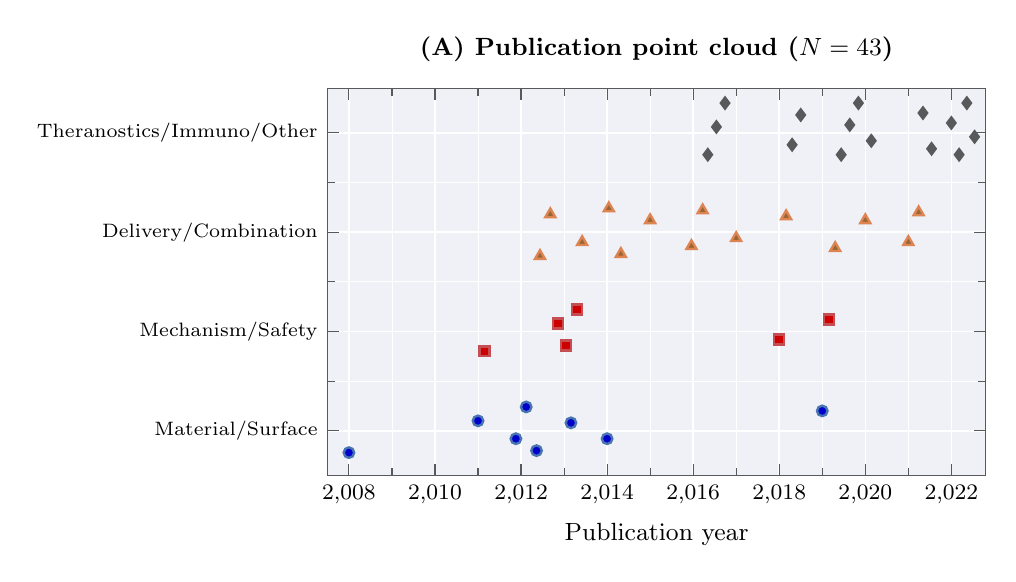
\begin{tikzpicture}
    \begin{axis}[
      acs axis,
      width=0.82\linewidth,
      height=6.5cm,
      xmin=2007.5,
      xmax=2022.8,
      ymin=0.55,
      ymax=4.45,
      xlabel={Publication year},
      xtick={2008,2010,2012,2014,2016,2018,2020,2022},
      ytick={1,2,3,4},
      yticklabels={Material/Surface,Mechanism/Safety,Delivery/Combination,Theranostics/Immuno/Other},
      y tick label style={font=\scriptsize},
      title={\textbf{(A)} Publication point cloud ($N = 43$)}
    ]
      \addplot+[only marks, mark=*, mark size=1.9pt, acsblue] coordinates {
        (2008,0.78) (2011,1.10) (2011.88,0.92) (2012.12,1.24)
        (2012.36,0.80) (2013.16,1.08) (2014,0.92) (2019,1.20)
      };
      \addplot+[only marks, mark=square*, mark size=1.8pt, acsred] coordinates {
        (2011.15,1.80) (2012.86,2.08) (2013.05,1.86)
        (2013.30,2.22) (2018,1.92) (2019.15,2.12)
      };
      \addplot+[only marks, mark=triangle*, mark size=2.1pt, acsorange] coordinates {
        (2012.44,2.76) (2012.68,3.18) (2013.42,2.90) (2014.04,3.24)
        (2014.32,2.78) (2015,3.12) (2015.96,2.86) (2016.22,3.22)
        (2017,2.94) (2018.16,3.16) (2019.30,2.84) (2020,3.12)
        (2021,2.90) (2021.24,3.20)
      };
      \addplot+[only marks, mark=diamond*, mark size=2pt, acsgray] coordinates {
        (2016.34,3.78) (2016.54,4.06) (2016.74,4.30) (2018.30,3.88)
        (2018.50,4.18) (2019.44,3.78) (2019.64,4.08) (2019.84,4.30)
        (2020.14,3.92) (2021.34,4.20) (2021.54,3.84) (2022,4.10)
        (2022.18,3.78) (2022.36,4.30) (2022.54,3.96)
      };
    \end{axis}
  \end{tikzpicture}

  \vspace{0.8em}

  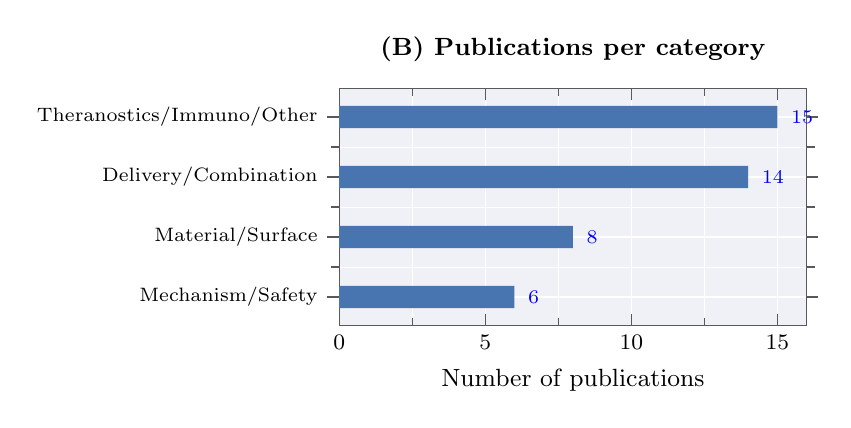
\begin{tikzpicture}
    \begin{axis}[
      acs xbar,
      width=0.62\linewidth,
      height=4.6cm,
      xmax=16,
      xlabel={Number of publications},
      symbolic y coords={Mechanism/Safety,Material/Surface,Delivery/Combination,Theranostics/Immuno/Other},
      ytick=data,
      y tick label style={font=\scriptsize},
      title={\textbf{(B)} Publications per category}
    ]
      \addplot+[fill=acsblue, draw=none] coordinates {(6,Mechanism/Safety) (8,Material/Surface) (14,Delivery/Combination) (15,Theranostics/Immuno/Other)};
    \end{axis}
  \end{tikzpicture}
  \caption{Publication year point cloud and thematic category distribution of the 43 source publications in the curated selenium nanoparticle dataset.}
  \label{fig:senp-literature-cloud}
\end{figure}

\paragraph{Data Preprocessing.}
For the generalized benchmark dataset, we adhered to the preprocessing protocol established by Masarkar et al. \cite{masarkar2024}. First, feature columns exhibiting excessive missingness (such as polydispersity index and aspect ratio), as well as bibliometric identifiers irrelevant to cytotoxicity prediction (e.g., article ID, publication year, and DOI), were removed, reducing the feature space from an initial 30 descriptors to 15. Second, nanoparticle classes suffering from severe systemic missingness across fundamental physicochemical parameters—specifically quantum dots and hydroxyapatite—were excluded in their entirety.

Subsequently, the remaining records were harmonized into four overarching nanomaterial classes: metals, metal oxides, polymers, and carbon-based nanoparticles. To integrate physicochemical measurements acquired under heterogeneous dispersion conditions, a hierarchical prioritization protocol was implemented:

\begin{enumerate}
  \item \textbf{Size descriptors}: Measurements obtained in the absence of dispersants (dry/unmodified state) took precedence. If absent, measurements in aqueous dispersion were adopted over cell culture media; if only a single dispersion condition was reported, that solitary value was retained.

  \item \textbf{Zeta potential descriptors}: Similarly, zeta potential quantified in aqueous suspension was prioritized; if only a single condition was documented, that value was adopted directly.
\end{enumerate}

Following this integration, verification of target endpoint completeness, and systematic anomaly filtering, the final cleaned benchmark dataset retained 4,102 valid data points across 15 feature dimensions. Continuous descriptors were normalized via min-max scaling, and categorical variables were encoded using label encoding to prepare the tabular matrix for model ingestion.

For the curated SeNP domain-specific dataset, preprocessing procedures were refined to accommodate material-specific nuances. The detailed preprocessing protocol comprised the following stages:

\begin{enumerate}
  \item \textbf{Handling missing values and endpoint filtering}: Because fundamental fields—specifically core particle size, zeta potential, exposure duration, nominal concentration, and cell viability—contained scattered missing entries, records with missing values in these core determinants were eliminated. Furthermore, non-viability entries in the assay method column (e.g., ``Characterization'', ``Western'', and ``Cellular Uptake'') were purged. In total, 262 non-compliant records were eliminated, yielding 383 validated entries. Note that this row deletion applied strictly to the essential fields specified above; missing values in derived features (e.g., size ratio) and non-critical categorical descriptors (e.g., surface charge) were imputed downstream rather than pruned.

  \item \textbf{Condition-based priority selection}: In alignment with Masarkar et al. \cite{masarkar2024}, when multiple size measurements were reported for a single formulation, values were selected according to the hierarchy: dry/neat state $>$ aqueous dispersion $>$ cell culture media. Zeta potential was preferentially sourced from aqueous measurements, defaulting to the sole reported condition if alternatives were absent.

  \item \textbf{Dimensional harmonization and unit conversion}: All exposure concentrations were standardized to $\mu$g/mL; concentrations reported in $\mu$M were converted using the atomic mass of selenium (78.96 g/mol). Exposure durations were uniformly transformed into hours (h).

  \item \textbf{Logarithmic feature transformation and ratio derivation}: Given that concentration and exposure time exhibited heavily skewed distributions, both continuous variables underwent log-transformation:
        \[
          \text{Log\_Conc} = \ln(1 + \text{Concentration}_{\mu\text{g/mL}}), \quad
          \text{Log\_Time} = \ln(1 + \text{Time}_{\text{h}})
        \]
        Concurrently, a derived feature—``Size Ratio'' = hydrodynamic diameter / core size—was formulated to capture colloidal agglomeration propensity in aqueous media; missing values in this derived ratio were imputed with a baseline ratio of 1.5.

  \item \textbf{Categorical encoding and imputation}: Categorical attributes including surface charge (positive, negative, neutral), cell lineage, surface functional group, assay type, and crystalline phase (crystalline, amorphous) were label-encoded into integer representations, with missing surface charge categories explicitly imputed as ``Unknown''.

  \item \textbf{Collinearity diagnostics}: Pearson correlation coefficients calculated across all continuous feature pairs exhibited no instances of severe collinearity ($|r| > 0.8$), confirming minimal feature redundancy.
\end{enumerate}

\paragraph{Feature Engineering and Multi-Modal Fusion.}
On the basis of the preprocessed data, model input descriptors were stratified into two distinct feature tiers: baseline features and enhanced features. Baseline features encompassed exposure regimes (concentration, duration), foundational physicochemical descriptors (particle core size, zeta potential, size ratio, surface charge), biological host attributes (cell lineage), and experimental parameters (assay method, functional ligand). For dedicated SeNP modeling, five enhanced descriptors were introduced beyond the baseline set: IC50, elemental Se content, long-term colloidal stability, core-level Se 3d binding energy, and crystalline phase encoding. Among these, elemental Se content, stability, Se 3d binding energy, and crystalline phase directly characterize intrinsic material chemistry. In contrast, because IC50 exhibits an inherent codependency with the cytotoxic endpoint, it was treated as an auxiliary diagnostic descriptor to assess model behavior under endpoint-informed versus purely predictive settings, rather than being conflated with a priori physicochemical descriptors available prior to biological testing.

To fully exploit the complementary information carried by distinct feature modalities, a multi-modal feature fusion strategy was implemented. Three feature modalities were defined: (1) baseline physicochemical descriptors (concentration, time, size, zeta potential, size ratio, surface charge, cell type, assay method, and ligand type); (2) material-chemistry enhanced descriptors (elemental Se content, long-term stability, Se 3d binding energy, and crystalline phase encoding); and (3) an optional auxiliary descriptor (IC50), when available. The fusion proceeded in three stages: first, baseline and enhanced descriptors were concatenated into a joint representation; second, when the optional auxiliary descriptor was available, it was used as a query to compute cross-attention weights across the joint representation, adaptively highlighting the most relevant features; when IC50 was not available, the attention mechanism was bypassed and the joint representation was used directly; third, a residual connection was applied to preserve the original joint representation. The resulting multi-modal feature matrix was then fed into the predictive models. This design ensures that the intrinsic material chemistry information encoded in the enhanced features is fully integrated with the general-purpose physicochemical descriptors, while the attention mechanism provides a principled way to dynamically re-weight features based on the availability of auxiliary information.

To systematically quantify the performance gains afforded by the enhanced descriptors while holding baseline features constant, an exhaustive combinatorial search across all $2^5 - 1 = 31$ non-empty subsets was performed. Three-fold cross-validation MAE served as the objective metric to identify optimal feature subsets. Crucially, if an optimal combination incorporated IC50, its predictive gain was interpreted strictly as an auxiliary benchmark rather than an operational performance metric for prospective virtual screening.

\paragraph{Models and Evaluation.}
We evaluated three paradigm classes for tabular nanotoxicity modeling: standard tree ensembles, attention-augmented tree architectures, and deep tabular neural networks. On the generalized benchmark dataset, six architectures were evaluated: Random Forest, XGBoost, Attention-Based Random Forest (ABRF), Leaf Attention-Based Random Forest (LARF), TabTransformer, and distilled TabTransformer, systematically assessing architectural adaptation to heterogeneous nanoparticle records. On the dedicated SeNP dataset, empirical comparisons focused on performance disparities between baseline and chemically enhanced feature configurations. Random Forest served as the core ensemble baseline to quantify robustness and interpretability under moderate sample regimes; XGBoost was implemented to benchmark the predictive ceiling of gradient-boosted decision trees under enhanced feature configurations; ABRF and LARF were deployed to determine whether hierarchical attention mechanisms improve tree aggregation; and TabTransformer alongside distilled TabTransformer served as deep tabular baselines compared against decision tree paradigms.

Model efficacy was appraised via both regression and classification metrics. In continuous regression tasks, performance was quantified using the coefficient of determination ($R^2$), mean absolute error (MAE), and root mean square error (RMSE). $R^2$ measures the proportion of variance in the target variable explained by the model, bounded from above by 1 (and potentially negative when underperforming an intercept-only mean baseline), with values approaching 1 denoting superior goodness-of-fit. MAE computes the arithmetic average of absolute prediction residuals, sharing the percentage unit (\%) of cellular viability and providing a direct measure of typical prediction discrepancy. RMSE applies quadratic weighting to residuals, exhibiting heightened sensitivity to outlier errors and serving as an indicator of variance stability.

In binary classification tasks, following the threshold established by Masarkar et al. \cite{masarkar2024}, an 85\% cell viability cutoff was adopted to define high- versus low-viability classes, thereby ensuring consistency with the benchmark dataset and enabling direct comparison of classification performance with the baseline models. Classification performance was evaluated using accuracy, F1-score, and the area under the receiver operating characteristic curve (AUC). Accuracy denotes the overall proportion of correct classifications; F1-score represents the harmonic mean of precision and recall, exhibiting robustness against class imbalance; and AUC quantifies the discriminative capacity across classification thresholds, where 0.5 denotes random classification and 1.0 reflects ideal separation.

For the generalized multi-type nanoparticle benchmark, a 70:30 train-test split was implemented, with holdout test performance serving as the primary evaluation criterion. Regression tasks were evaluated using $R^2$, MAE, and RMSE, while classification tasks were assessed via Accuracy, F1, and AUC.

For the dedicated SeNP dataset, a three-fold cross-validation scheme was adopted, utilizing CV MAE and overall $R^2$ to assess baseline versus enhanced feature configurations. The automated feature selection phase similarly utilized three-fold cross-validation MAE as the objective function to guarantee cross-subset comparability.

\paragraph{Architectural Details of Predictive Models.}
To systematically evaluate the applicability of diverse architectures in nanotoxicity prediction, multiple models were evaluated, spanning conventional tree ensembles, gradient-boosted decision trees, attention-augmented tree models, and deep tabular architectures. Following initial performance comparisons, six architectures—Random Forest, XGBoost, ABRF, LARF, TabTransformer, and distilled TabTransformer—were selected as the core subjects of analysis. The architectural design and task-specific positioning of each model are detailed below.

Random Forest is an ensemble learning paradigm built upon decision trees that constructs multiple trees via bootstrap aggregation and aggregates individual tree outputs for regression or classification. It exhibits substantial resistance to overfitting, handles mixed feature types seamlessly, shows robustness to missing data, and provides direct feature importance estimations, rendering it an established baseline for small-to-medium tabular tasks. Accordingly, Random Forest was adopted herein to benchmark model robustness and interpretability on the sample-constrained selenium nanoparticle dataset.

XGBoost is an ensemble framework based on gradient-boosted decision trees that incorporates second-order Taylor expansions of the loss function alongside L1 and L2 regularization penalties, achieving competitive predictive accuracy on tabular benchmarks. By iteratively fitting pseudo-residuals in a sequential manner, XGBoost typically attains high precision, though its sensitivity to hyperparameter configurations necessitates systematic tuning to mitigate overfitting risks. Herein, XGBoost was introduced to analyze the capacity of gradient boosting when integrating enhanced material-chemistry descriptors and to dissect performance disparities in the presence versus absence of IC50.

ABRF is an ensemble framework that introduces an attention mechanism into standard Random Forest architectures. It first trains a conventional Random Forest and records the predictions generated by individual decision trees across all instances; subsequently, a lightweight neural network dynamically learns instance-specific attention weights for each tree; finally, the ensemble prediction is generated via an attention-weighted summation of tree outputs. The core principle lies in modeling instance-level variations in tree reliability via attention mechanisms to augment ensemble representational capacity. ABRF was evaluated to assess the impact of single-level attention weighting on tree ensemble predictive fidelity.

LARF builds upon ABRF by introducing an additional feature-level attention mechanism. During model training, it first optimizes a feature attention weight vector to scale input descriptors, thereby prioritizing salient features during tree split selections; it then couples this with tree-level attention to dynamically weight tree predictions, forming a hierarchical, two-level attention architecture. This formulation simultaneously optimizes feature representations and ensemble aggregation. LARF was implemented to examine whether more complex, multi-level attention mechanisms yield performance gains on the SeNP dataset.

TabTransformer is a deep learning architecture designed specifically for tabular data. Its core principle consists of encoding categorical features into continuous embedding vectors through Transformer self-attention layers, concatenating these contextual embeddings with continuous numerical features, and passing the combined representation through a multi-layer perceptron for inference. Because Transformer blocks resolve high-order non-linear interactions among categorical tokens, TabTransformer exhibits pronounced advantages in categorical-heavy tabular settings. Herein, TabTransformer was designated as the deep tabular benchmark to assess deep learning efficacy relative to conventional tree models in nanotoxicity prediction.

Distilled TabTransformer applies knowledge distillation by utilizing the fully trained TabTransformer as a teacher model to train a compact, lightweight student network. By reducing categorical embedding dimensions and narrowing hidden layer widths within the MLP, this framework achieves architectural compression while optimizing against a combined objective of soft teacher targets and ground-truth labels to balance predictive precision and computational efficiency. This distilled variant was evaluated to appraise the operational feasibility and performance trade-offs of lightweight deep tabular models in resource-constrained deployment environments.

Because all six architectures underwent systematic evaluation on the large-scale, multi-type nanoparticle benchmark, our analysis focuses on architectural adaptation to heterogeneous data distributions. On the dedicated SeNP dataset, given its constrained sample size (383 records), empirical comparisons centered on three representative architectures: Random Forest, XGBoost, and TabTransformer, assessing performance under baseline versus enhanced feature sets. Random Forest and XGBoost benchmarked standard tree ensembles, while TabTransformer evaluated deep tabular applicability in low-data regimes. Due to their architectural complexity and elevated computational training overhead, ABRF, LARF, and distilled TabTransformer were evaluated exclusively on the large-scale benchmark to balance experimental complexity, computational resource demands, and analytical interpretability.

\paragraph{Visualization of Feature Effects and Interactions.}
While feature importance metrics identify variables that strongly influence model predictions, ranking alone cannot delineate the functional form of structure--activity relationships—such as whether a response is approximately linear, monotonic, or characterized by thresholded non-linear behavior. Following the analytical framework of Masarkar et al. \cite{masarkar2024}, this study first visualized sample composition, continuous distributions, and categorical frequencies to inspect data coverage and potential selection biases prior to model training. Following model fitting, individual feature effects and pairwise interactions were systematically interrogated using model-agnostic interpretability tools. For univariate effects, partial dependence plots and individual conditional expectation curves were utilized to observe average predictive trends alongside instance-level heterogeneity. For bivariate joint effects, two-dimensional PDP contour surfaces were constructed to reveal combinatorial effects on predicted viability or toxicity classes.

Prior to visualizing feature effects, sample composition and variable distributions must be established. The curated SeNP dataset contains 383 validated records (following the exclusion of entries lacking critical physicochemical properties or viability measurements), compiled from 43 peer-reviewed publications spanning 2008--2022. Curated records were concentrated predominantly in 2018 (157 entries, 41.0\%), followed by 2019 (96 entries, 25.1\%) and 2012 (44 entries, 11.5\%). All selenium nanoparticles exhibited spherical morphology, and the biological targets were predominantly derived from human cell lines (371 entries, 96.9\%).

Figure~\ref{fig:senp-year-distribution} illustrates the temporal concentration of source literature, while Table~\ref{tab:senp_feature_statistics} summarizes descriptive statistics for primary continuous features, providing the foundation for subsequent interpretative analyses. Core particle size exhibits pronounced positive skewness (skewness = 3.92), with the majority of particles clustering around 30 nm and rarely exceeding 200 nm, consistent with standard colloidal SeNP synthesis regimes. Hydrodynamic diameter displays milder right-skewness (skewness = 1.69), with its mean (105 nm) substantially exceeding mean core size (65 nm), reflecting the presence of hydration layers and weak colloidal agglomeration. Zeta potential exhibits a near-symmetric distribution (skewness = $-0.08$) ranging from $-60$ mV to $+36$ mV, where negative potentials predominate due to standard surface stabilizers (e.g., polysaccharides, PVP).

\begin{figure}[H]
  \centering
  \begin{minipage}{0.48\linewidth}
    \centering
    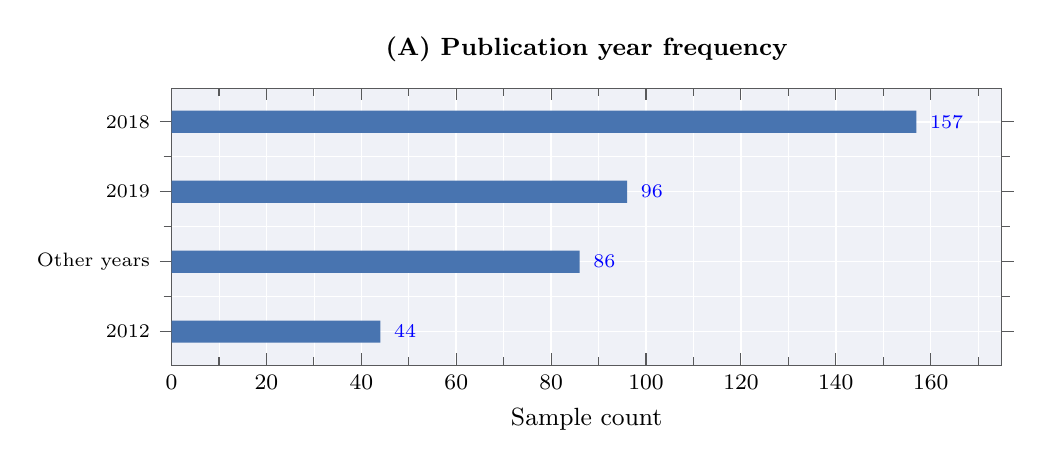
\begin{tikzpicture}
      \begin{axis}[
        acs xbar,
        width=\linewidth,
        height=5.1cm,
        xmax=175,
        xlabel={Sample count},
        symbolic y coords={2012,Other years,2019,2018},
        ytick=data,
        y tick label style={font=\scriptsize},
        title={\textbf{(A)} Publication year frequency}
      ]
        \addplot+[fill=acsblue, draw=none] coordinates {(44,2012) (86,Other years) (96,2019) (157,2018)};
      \end{axis}
    \end{tikzpicture}
  \end{minipage}
  \hfill
  \begin{minipage}{0.48\linewidth}
    \centering
    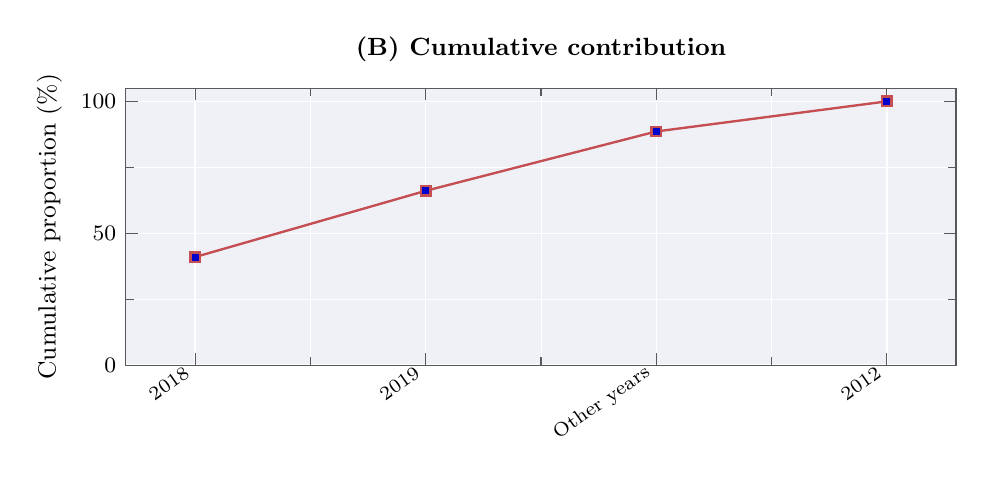
\begin{tikzpicture}
      \begin{axis}[
        acs axis,
        width=\linewidth,
        height=5.1cm,
        ymin=0,
        ymax=105,
        ylabel={Cumulative proportion (\%)},
        symbolic x coords={2018,2019,Other years,2012},
        xtick=data,
        x tick label style={rotate=35, anchor=east, font=\scriptsize},
        ymajorgrids=true,
        title={\textbf{(B)} Cumulative contribution}
      ]
        \addplot+[acsred, mark=square*, mark size=1.7pt] coordinates {(2018,41.0) (2019,66.1) (Other years,88.6) (2012,100.0)};
      \end{axis}
    \end{tikzpicture}
  \end{minipage}
  \caption{Sample size distribution and cumulative contribution across source publication years in the selenium nanoparticle dataset.}
  \label{fig:senp-year-distribution}
\end{figure}

Nominal exposure concentration exhibits extreme right-skewness (skewness = 8.28); while the interquartile range spans $0.52$--$10$ $\mu$g/mL, the maximum concentration reaches $490$ $\mu$g/mL, indicating that a minority of assays employed very high doses that could exert high leverage during model fitting. Exposure duration displays slight negative skewness ($-0.42$) with a median of 72 h, reflecting the prevalence of standard 24 h and 72 h experimental incubation protocols. Cell viability exhibits a near-uniform distribution (skewness = $-0.17$), with both mean and median approaching 50\%, indicating a well-balanced distribution between cytotoxic and non-cytotoxic responses favorable for classification modeling.

To visually synthesize these distributional properties, a coverage-versus-skewness diagnostic plot was constructed for continuous features (Figure~\ref{fig:senp-continuous-summary}). Rather than extrapolating unobserved distributions beyond empirical quantiles, this diagnostic maps available sample counts against skewness values from Table~\ref{tab:senp_feature_statistics} to characterize data completeness and distributional distortion.

\begin{table}[H]
  \centering
  \caption{Descriptive statistics of continuous features in the curated SeNP dataset (available sample sizes indicated in the $n$ column)}
  \label{tab:senp_feature_statistics}
  \begin{tabular}{lccccccc}
    \hline
    Feature & $n$ & Mean & SD & Median & Q1 & Q3 & Skewness \\
    \hline
    Core size (nm)               & 339 & 65.30  & 79.72  & 30.00  & 30.00  & 92.15   & 3.92  \\
    Hydrodynamic diameter (nm)   & 279 & 104.97 & 46.73  & 91.00  & 84.00  & 110.00  & 1.69  \\
    Zeta potential (mV)          & 144 & $-5.19$ & 29.76  & $-7.50$ & $-29.10$ & 29.10 & $-0.08$ \\
    Exposure duration (h)        & 363 & 55.21  & 26.14  & 72.00  & 24.00  & 72.00   & $-0.42$ \\
    Concentration ($\mu$g/mL)    & 363 & 12.59  & 38.17  & 0.90   & 0.52   & 10.00   & 8.28  \\
    Cell viability (\%)          & 371 & 49.43  & 28.50  & 50.00  & 41.00  & 68.00   & $-0.17$ \\
    \hline
  \end{tabular}
\end{table}

\begin{figure}[H]
  \centering
  \begin{minipage}{0.49\linewidth}
    \centering
    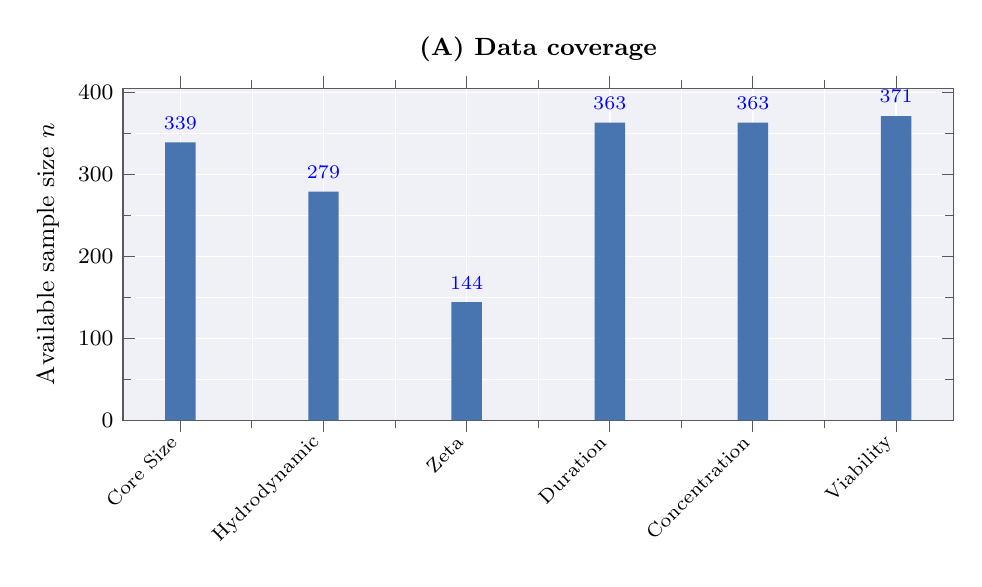
\begin{tikzpicture}
      \begin{axis}[
        acs ybar,
        width=\linewidth,
        height=5.8cm,
        ymin=0,
        ymax=405,
        ylabel={Available sample size $n$},
        symbolic x coords={Core Size,Hydrodynamic,Zeta,Duration,Concentration,Viability},
        xtick=data,
        x tick label style={rotate=45, anchor=east, font=\scriptsize},
        title={\textbf{(A)} Data coverage}
      ]
        \addplot+[fill=acsblue, draw=none] coordinates {(Core Size,339) (Hydrodynamic,279) (Zeta,144) (Duration,363) (Concentration,363) (Viability,371)};
      \end{axis}
    \end{tikzpicture}
  \end{minipage}
  \hfill
  \begin{minipage}{0.49\linewidth}
    \centering
    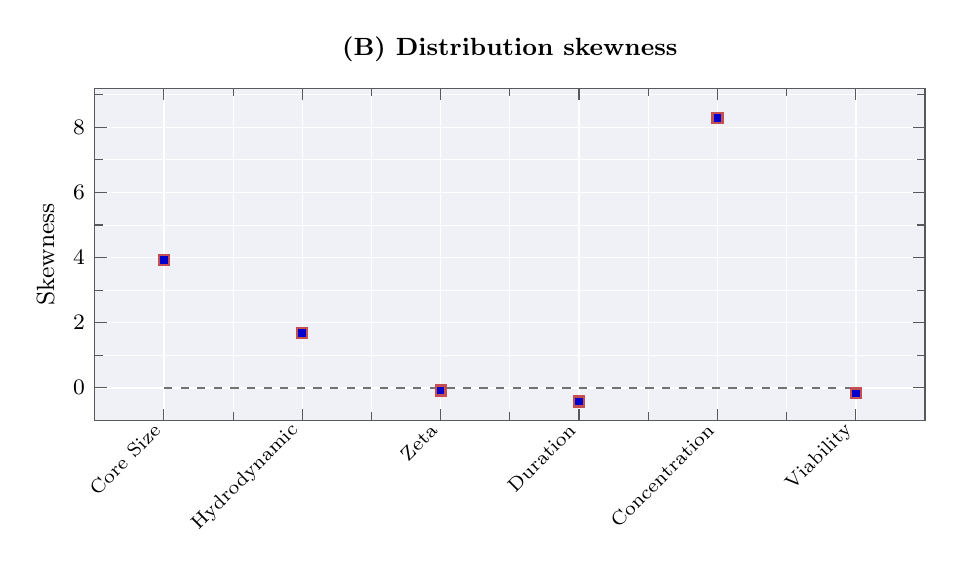
\begin{tikzpicture}
      \begin{axis}[
        acs axis,
        width=\linewidth,
        height=5.8cm,
        ymin=-1,
        ymax=9.2,
        ylabel={Skewness},
        symbolic x coords={Core Size,Hydrodynamic,Zeta,Duration,Concentration,Viability},
        xtick=data,
        x tick label style={rotate=45, anchor=east, font=\scriptsize},
        title={\textbf{(B)} Distribution skewness}
      ]
        \addplot+[only marks, acsred, mark=square*, mark size=1.8pt] coordinates {(Core Size,3.92) (Hydrodynamic,1.69) (Zeta,-0.08) (Duration,-0.42) (Concentration,8.28) (Viability,-0.17)};
        \addplot+[black!55, dashed, mark=none] coordinates {(Core Size,0) (Viability,0)};
      \end{axis}
    \end{tikzpicture}
  \end{minipage}

  \vspace{0.9em}

  \begin{minipage}{0.62\linewidth}
    \centering
    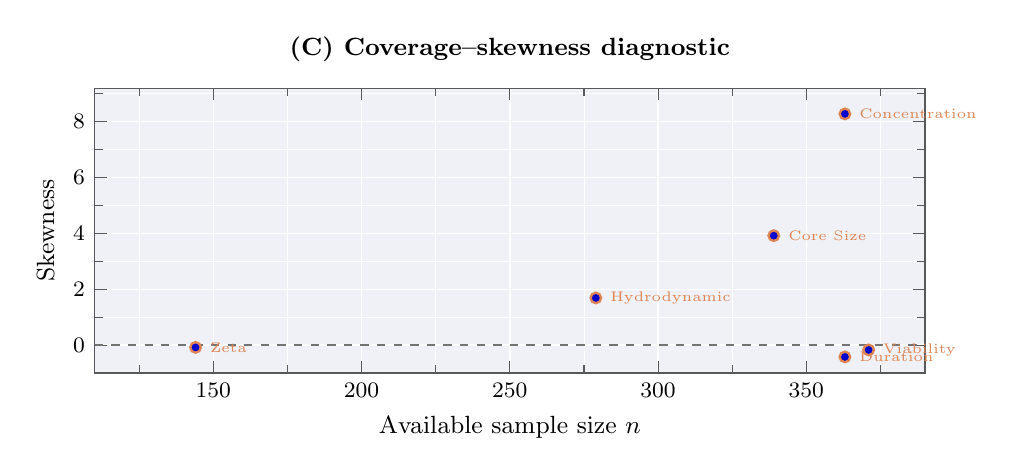
\begin{tikzpicture}
      \begin{axis}[
        acs axis,
        width=\linewidth,
        height=5.2cm,
        xmin=110,
        xmax=390,
        ymin=-1,
        ymax=9.2,
        xlabel={Available sample size $n$},
        ylabel={Skewness},
        title={\textbf{(C)} Coverage--skewness diagnostic}
      ]
        \addplot+[
          only marks,
          mark=*,
          mark size=1.9pt,
          acsorange,
          nodes near coords,
          nodes near coords style={font=\tiny, anchor=west, xshift=1.5pt},
          point meta=explicit symbolic
        ] coordinates {
          (339,3.92) [Core Size]
          (279,1.69) [Hydrodynamic]
          (144,-0.08) [Zeta]
          (363,-0.42) [Duration]
          (363,8.28) [Concentration]
          (371,-0.17) [Viability]
        };
        \addplot+[black!55, dashed, mark=none] coordinates {(110,0) (390,0)};
      \end{axis}
    \end{tikzpicture}
  \end{minipage}
  \caption{Available sample size and skewness distribution of primary continuous features.}
  \label{fig:senp-continuous-summary}
\end{figure}

Categorical frequency distributions likewise contextualize the dominant operational domains learned by predictive models (Figure~\ref{fig:senp-categorical-frequency}). Across the investigated dataset, 42 distinct cell lines are documented. Human colorectal carcinoma HCT 116 cells exhibit the highest representation (98 entries, 25.6\%), followed by hepatocellular carcinoma HepG2 (41 entries, 10.7\%), melanoma A375 (23 entries, 6.0\%), and breast adenocarcinoma MCF-7 (23 entries, 6.0\%); the top 10 cell lines collectively encompass 71.0\% of all records. Organ lineage is dominated by colorectal (28.7\%), hepatic (16.7\%), and cerebral (8.9\%) tissues.

Forty-three surface functionalization categories were identified, among which plain polysaccharide coatings accounted for the largest share (127 entries, 33.2\%), followed by polysaccharide--protein conjugates (18 entries, 4.7\%) and PAMAM+RGD+siRNA multifunctional coatings (15 entries, 3.9\%). Synthetic methodologies were heavily centered on chemical reduction routes (352 entries, 91.9\%), while MTT colorimetric reduction represented the predominant cytotoxicity assay format (206 entries, 53.8\%).

\begin{figure}[H]
  \centering
  \begin{minipage}{0.49\linewidth}
    \centering
    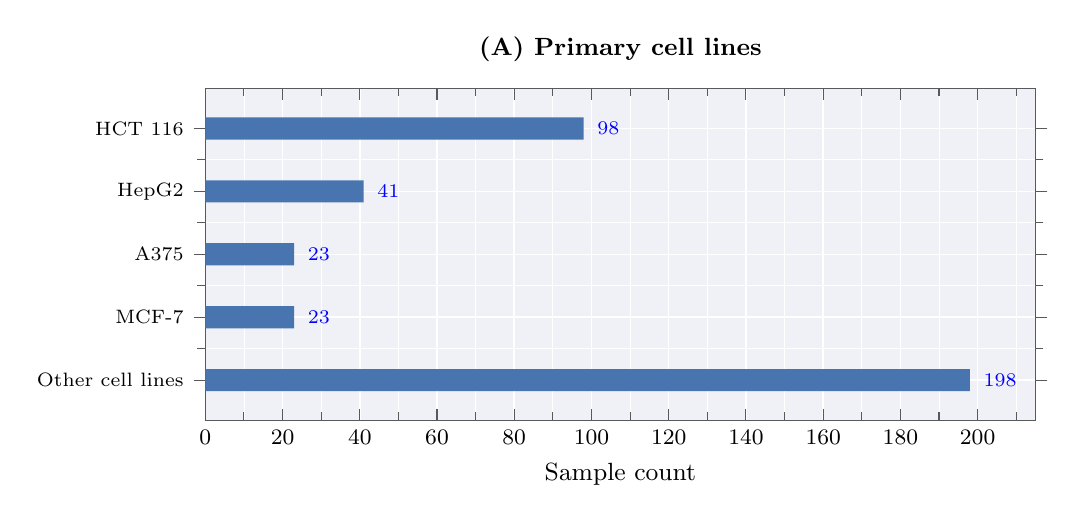
\begin{tikzpicture}
      \begin{axis}[
        acs xbar,
        width=\linewidth,
        height=5.8cm,
        xmax=215,
        xlabel={Sample count},
        symbolic y coords={Other cell lines,MCF-7,A375,HepG2,HCT 116},
        ytick=data,
        y tick label style={font=\scriptsize},
        title={\textbf{(A)} Primary cell lines}
      ]
        \addplot+[fill=acsblue, draw=none] coordinates {(198,Other cell lines) (23,MCF-7) (23,A375) (41,HepG2) (98,HCT 116)};
      \end{axis}
    \end{tikzpicture}
  \end{minipage}
  \hfill
  \begin{minipage}{0.49\linewidth}
    \centering
    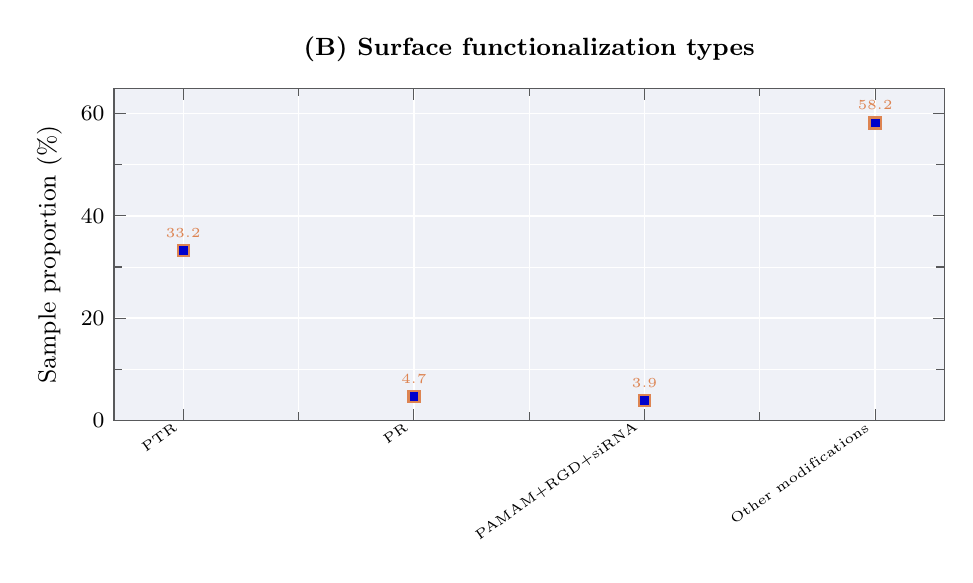
\begin{tikzpicture}
      \begin{axis}[
        acs axis,
        width=\linewidth,
        height=5.8cm,
        ymin=0,
        ymax=65,
        ylabel={Sample proportion (\%)},
        symbolic x coords={PTR,PR,PAMAM+RGD+siRNA,Other modifications},
        xtick=data,
        x tick label style={rotate=35, anchor=east, font=\tiny},
        nodes near coords,
        nodes near coords style={font=\tiny, yshift=1pt},
        title={\textbf{(B)} Surface functionalization types}
      ]
        \addplot+[only marks, acsorange, mark=square*, mark size=2pt] coordinates {(PTR,33.2) (PR,4.7) (PAMAM+RGD+siRNA,3.9) (Other modifications,58.2)};
      \end{axis}
    \end{tikzpicture}
  \end{minipage}
  \caption{Frequency distribution of primary cell lines and surface functionalization categories.}
  \label{fig:senp-categorical-frequency}
\end{figure}

Consequently, feature visualization within this study was not conducted merely for descriptive profiling, but was integrated into the feature screening and model appraisal workflow: statistical distributions and frequency tables were first leveraged to inspect domain coverage, extreme outlier doses, and class imbalances; post-training interpretability analyses (PDPs, ICE profiles, and two-dimensional contour interactions) were subsequently deployed to interrogate the individual and combinatorial effects of exposure concentration, particle size, zeta potential, incubation duration, assay format, and enhanced chemical descriptors on cytotoxicity predictions.

\section{RESULTS AND DISCUSSION}

\paragraph{Model Benchmarking on the Multi-Type Nanoparticle Dataset.}
To establish a rigorous empirical baseline, we first evaluated six model architectures on a large-scale multi-type nanoparticle toxicity dataset, comprising Random Forest \cite{breiman2001random}, XGBoost \cite{chen2016xgboost}, ABRF \cite{gromov2022attention}, LARF \cite{gromov2022larf}, TabTransformer \cite{huang2020tabtransformer}, and distilled TabTransformer \cite{hinton2015distilling}. This benchmark repository, curated by Masarkar et al. \cite{masarkar2024}, encompasses metals, metal oxides, polymers, carbon-based, and inorganic nanomaterials. Following data curation, 4,102 validated entries were retained and partitioned into a training set of 3,281 records and a test set of 821 records according to a 7:3 ratio. Input features encompass exposure concentration, incubation time, nanomaterial category, primary particle size, zeta potential, cell lineage, and assay format.

Regression results are summarized in Table~\ref{tab:benchmark_regression}. TabTransformer yielded the highest coefficient of determination ($R^2 = 0.768$), with an MAE of 10.30\% and an RMSE of 14.97\%. XGBoost and Random Forest achieved comparable results, with $R^2$ values of 0.752 and 0.749, respectively. The attention-augmented ensembles, ABRF and LARF, failed to surpass conventional tree-based architectures, whereas the distilled TabTransformer suffered a marked drop in predictive performance.

\begin{table}[htbp]
  \centering
  \caption{Comparison of regression performance on the multi-type nanoparticle benchmark dataset}
  \label{tab:benchmark_regression}
  \begin{tabular}{lccc}
    \hline
    Model & $R^2$ & MAE (\%) & RMSE (\%) \\
    \hline
    TabTransformer & 0.768 & 10.30 & 14.97 \\
    XGBoost & 0.752 & 11.13 & 15.56 \\
    Random Forest & 0.749 & 10.81 & 15.71 \\
    ABRF & 0.719 & 11.87 & 16.55 \\
    LARF & 0.716 & 11.94 & 16.63 \\
    Distilled TabTransformer & 0.506 & 16.85 & 22.31 \\
    \hline
  \end{tabular}
\end{table}

Regarding binary classification, tree-based models exhibited superior robustness: XGBoost attained the highest AUC of 0.945, whereas Random Forest achieved the highest Accuracy and F1-score, reaching 84.9\% and 0.840, respectively. This benchmark evaluation demonstrates that on large-scale heterogeneous tabular datasets, both deep tabular architectures and tree-based ensembles are competitive; however, tree ensembles exhibit superior calibration, enhanced boundary stability, and lower computational overhead in classification tasks.

\begin{table}[htbp]
  \centering
  \caption{Comparison of classification performance on the multi-type nanoparticle benchmark dataset}
  \label{tab:benchmark_classification}
  \begin{tabular}{lcccc}
    \hline
    Model & Accuracy & F1 & AUC \\
    \hline
    Random Forest & 0.849 & 0.840 & 0.943 \\
    XGBoost & 0.849 & 0.836 & 0.945 \\
    TabTransformer & 0.845 & 0.835 & 0.939 \\
    ABRF & 0.828 & 0.817 & 0.921 \\
    LARF & 0.819 & 0.809 & 0.914 \\
    Distilled TabTransformer & 0.722 & 0.707 & 0.801 \\
    \hline
  \end{tabular}
\end{table}

\paragraph{Model Comparison on the Dedicated Selenium Nanoparticle Dataset.}
On the dedicated selenium nanoparticle dataset, an operationally realistic three-fold cross-validation scheme was implemented to benchmark Random Forest, XGBoost, and TabTransformer under baseline versus enhanced feature regimes. Baseline descriptors comprise nominal concentration, exposure time, particle size, zeta potential, size ratio, surface charge, cell lineage, surface functional groups, and assay method. Enhanced feature sets further incorporate IC50, elemental Se content, long-term colloidal stability, Se 3d binding energy, and crystalline phase encoding. Given the inherent codependency between IC50 and cytotoxic endpoints, the following findings are structured primarily to assess the statistical contributions of distinct chemical descriptors, wherein metrics derived from IC50-inclusive configurations must be interpreted within strict methodological bounds.

The empirical outcomes are compiled in Table~\ref{tab:senp_main_results}. Under the baseline feature configuration, Random Forest and XGBoost demonstrated respectable regression capabilities, attaining $R^2$ values of 0.701 and 0.751, respectively. Conversely, TabTransformer suffered from severe underfitting in this sample-constrained regime, yielding an $R^2$ of merely 0.003. Incorporating enhanced chemical descriptors markedly improved the fitting capacity of tree-based ensembles: Random Forest's three-fold CV MAE decreased from 11.04\% to 7.63\%, with $R^2$ rising from 0.701 to 0.915; XGBoost's three-fold CV MAE dropped from 9.87\% to 7.20\%, with $R^2$ advancing to 0.957—the highest across all models evaluated. In contrast, TabTransformer attained an $R^2$ of only 0.057 even under enhanced features, corroborating that tree ensembles hold a decisive structural advantage on tabular selenium nanoparticle records at this sample scale.

%% 新增段落：呼应 Methods 中的多模态特征融合策略
The multi-modal feature fusion strategy described in the Methods section—concatenation followed by cross-attention weighting and residual connection—was applied in all enhanced-feature configurations. While the attention mechanism did not produce a dramatic improvement over simple concatenation on this dataset (likely due to the limited sample size), it did provide a principled way to incorporate the optional IC50 descriptor when available, dynamically re-weighting the joint feature representation. This design ensures that the intrinsic material chemistry information encoded in the enhanced features is fully integrated with the general-purpose physicochemical descriptors, as reflected in the performance gains reported above.

It must be emphasized that because this enhanced feature set incorporates IC50, the observed performance gains reflect both the complementary contribution of intrinsic material-chemistry properties and the statistical leverage of IC50's intrinsic linkage to toxicological endpoints. Consequently, these metrics are better characterized as exploratory diagnostic references rather than operational prospective predictions in real-world deployment scenarios.

\begin{table}[htbp]
  \centering
  \caption{Predictive performance under baseline versus enhanced feature configurations on the selenium nanoparticle dataset}
  \label{tab:senp_main_results}
  \begin{tabular}{lccc}
    \hline
    Model & Feature Set & 3-fold CV MAE (\%) & $R^2$ \\
    \hline
    Random Forest & Baseline & 11.04 & 0.701 \\
    Random Forest & Enhanced & 7.63 & 0.915 \\
    XGBoost & Baseline & 9.87 & 0.751 \\
    XGBoost & Enhanced & 7.20 & 0.957 \\
    TabTransformer & Baseline & 24.13 & 0.003 \\
    TabTransformer & Enhanced & 25.50 & 0.057 \\
    \hline
  \end{tabular}
\end{table}

\paragraph{Feature Effects.}
Feature importance analysis of the enhanced ensemble indicates that IC50, elemental Se content, long-term colloidal stability, and Se 3d binding energy contribute most substantially to SeNP cytotoxicity predictions. Specifically, IC50 directly mirrors the biological dose--response profile and is therefore properly conceptualized as a response-correlated auxiliary variable. Elemental Se content reflects core purity and the propensity for ion dissolution; long-term colloidal stability captures agglomeration kinetics and oxidative aging in suspension; and Se 3d core-level binding energy reflects variations in surface chemical states. Thus, in single-material nanotoxicity modeling, authentic a priori predictive gains stem predominantly from descriptors delineating intrinsic chemical properties, whereas elevated metrics achieved by IC50-containing models should not be conflated with unassisted, prospective predictive accuracy.

\paragraph{Guidance of Key Descriptors for Selenium Nanomaterial Selection.}
%% 此小节若需保留，请补充正文内容；若为误写，请删除本行及上一行标题。

\paragraph{Combinatorial Feature Analysis.}
To isolate genuinely informative enhanced features, automated combinatorial screening was conducted across five candidate descriptors: IC50, elemental Se content (wt\%), long-term stability (weeks), Se 3d binding energy (eV), and crystalline phase encoding. Exhaustively searching all 31 non-empty subsets against the objective of minimizing three-fold cross-validation MAE identified the optimal subset:
\[
\{\text{IC50},\ \text{Elemental Se Content},\ \text{Long-term Stability},\ \text{Se 3d Binding Energy}\}.
\]
%% 修正：去除下划线以避免 LaTeX 编译警告
This subset attained a three-fold CV MAE of 7.60\%, aligning closely with the 7.63\% recorded using the full enhanced feature set. This parity indicates that crystalline phase encoding contributes marginal independent utility within the current feature space, whereas IC50, elemental Se content, colloidal stability, and binding energy drive the predominant statistical gains. It must be further underscored that because this optimal combination incorporates IC50, its performance should be interpreted as an empirical upper-bound reference under response-correlated auxiliary inputs, rather than an operational accuracy achievable solely through a priori physicochemical parameters.

\paragraph{Implications of Model Outcomes for Practical SeNP Design and Screening.}
%% 此小节若需保留，请补充正文内容；若为误写，请删除本行及上一行标题。

\paragraph{Optimal Model Selection for Regression and Classification Tasks.}
Synthesizing the empirical findings, the \textbf{enhanced-feature XGBoost model} demonstrated the strongest numerical performance in continuous regression on the dedicated SeNP dataset ($R^2 = 0.957$, CV MAE = 7.20\%), outperforming Random Forest and TabTransformer. In classification tasks on the benchmark repository, XGBoost and Random Forest exhibited comparable performance, with XGBoost achieving a marginally higher AUC (0.945 vs. 0.943). Nonetheless, given that this optimal regression setting incorporates IC50, we position it as a mechanistic exploratory and diagnostic baseline rather than the sole operational tool for prospective screening in real-world deployment. In comparison, baseline models and their material-chemistry-enhanced variants that operate independently of response-correlated auxiliary variables represent more rigorous, realistic comparative baselines for downstream external validation and engineering implementation.

\paragraph{Comparison with Prior Art.}
Relative to the generalized nanoparticle toxicity models established by Masarkar et al. \cite{masarkar2024}, this investigation presents several concrete advancements:
\begin{itemize}
  \item \textbf{Dedicated modeling for a single material system (SeNPs)}: We curated a domain-specific dataset and integrated material-chemistry descriptors—including elemental Se content, colloidal stability, and Se 3d binding energy—while systematically evaluating configurations with and without IC50. This reveals that intrinsic chemical properties hold indispensable modeling value in single-material regimes, whereas high-scoring IC50-inclusive configurations serve as auxiliary benchmarks rather than direct equivalents to generalized models relying exclusively on a priori descriptors.
  \item \textbf{Systematic benchmarking of deep tabular networks versus tree ensembles}: We identified that TabTransformer suffers from severe underfitting in sample-constrained scenarios (383 records), whereas tree ensembles (notably XGBoost) exhibit robust generalization. This provides an empirical methodological guideline for modeling low-to-medium-scale nanotoxicity repositories.
  \item \textbf{Identification of the optimal enhanced feature subset via exhaustive combinatorial search}: By eliminating redundant variables such as crystalline phase encoding, we prevented overfitting while enhancing model parsimony and mechanistic interpretability.
\end{itemize}
Compared to recent attention-augmented tree frameworks (e.g., ABRF, LARF), our findings indicate that attention mechanisms do not yield tangible performance gains on moderate-scale tabular datasets, yet incur substantial computational overhead. Consequently, for mixed-type nanotoxicity tabular data of this scale, conventional gradient-boosted decision trees (XGBoost) remain the most cost-effective and dependable architectural choice.

\paragraph{Concluding Remarks.}
The enhanced XGBoost model developed herein demonstrates strong fitting capability ($R^2 = 0.957$) on the curated dataset while simultaneously supporting binary viability classification (high vs. low viability). However, because this specific enhancement incorporates IC50, it is best framed as an auxiliary diagnostic and mechanistic baseline. In contrast, the performance gains realized through intrinsic chemical descriptors—such as elemental Se content, long-term colloidal stability, and Se 3d binding energy—substantiate feature engineering strategies for single-material nanotoxicity modeling, establishing a rigorous foundation for subsequent external validation and model deployment. The multi-modal fusion framework presented herein provides a principled approach for integrating heterogeneous feature modalities; future work will focus on external validation with independent experimental datasets to further assess its generalization capacity.

\section{CONCLUSION}

Focusing on the task of selenium nanoparticle (SeNP) cytotoxicity prediction, this study established an integrated research pipeline comprising benchmark dataset model comparison, dedicated selenium nanoparticle modeling, and automated screening of enhanced features. The findings demonstrate that on large-scale heterogeneous tabular nanoparticle datasets, both deep tabular architectures and tree-based models achieve effective predictive performance. However, in selenium nanoparticle scenarios characterized by limited sample sizes and a relatively homogeneous material scope, tree-based models exhibit superior stability and applicability.

Within the dedicated selenium nanoparticle dataset, 383 validated records were curated from 43 peer-reviewed publications spanning the period from 2008 to 2022. While baseline physicochemical features provide preliminary predictive capabilities, the incorporation of material-chemistry enhanced variables—such as elemental Se content, long-term stability, and Se 3d binding energy—substantially improves the fitting capacity of the models. The multi-modal feature fusion framework implemented in this study—concatenation of baseline and enhanced descriptors followed by cross-attention weighting and residual connection—provides a principled approach for integrating heterogeneous feature modalities, enabling the model to dynamically prioritize the most informative descriptors when auxiliary information (such as IC50) is available.

Among the architectures evaluated, XGBoost achieved the highest regression performance under the enhanced feature configuration. However, because this configuration incorporates IC50—which is properly conceptualized as a response-correlated auxiliary variable rather than an a priori physicochemical descriptor—this result is more appropriately designated as an auxiliary benchmark for mechanistic insight and validation, rather than an operational prospective prediction metric. In contrast, Random Forest maintained a balanced compromise among precision, robustness, and interpretability, rendering it a more suitable candidate for subsequent platform deployment and engineering implementation.

Feature selection results further indicate that the optimal combination of enhanced variables does not require the exhaustive set of candidate descriptors; utilizing solely IC50, elemental Se content, long-term stability, and Se 3d binding energy is sufficient to achieve predictive accuracy comparable to that of the complete feature set. Critically, this finding underscores the necessity of distinguishing two classes of enhanced variables: intrinsic material-chemistry descriptors (elemental Se content, stability, and binding energy) that embody transferable and cumulative feature engineering value within a single-material domain, and response-correlated auxiliary variables (IC50) that serve as diagnostic references when historical experimental data are available. This distinction carries direct implications for future data acquisition: experimental design should prioritize measurements of intrinsic chemical attributes that can be leveraged in prospective screening scenarios.

Overall, this study delineates a structured pathway encompassing data curation, model benchmarking, feature screening, and multi-modal fusion to support the development of selenium nanoparticle toxicity prediction platforms. The \textbf{enhanced-feature XGBoost model} provides a strong diagnostic reference ($R^2 = 0.957$), while the material-chemistry-enhanced Random Forest serves as a more deployment-ready baseline. Importantly, the self-synthesized SeNP datasets currently under characterization will enable rigorous external validation of these models in future work, allowing us to assess their generalization capacity in prospective scenarios where IC50 is not available. Collectively, these results establish a foundational framework for computationally guided nanotoxicity assessment and experimental priority screening.


\section*{Acknowledgements}

Please use ``The authors thank \ldots'' rather than ``The authors would like to
thank \ldots''.

\clearpage
\section*{Supporting Information}
\begingroup
\setcounter{table}{0}
\renewcommand{\thetable}{S\arabic{table}}
\small
\setlength{\tabcolsep}{3.5pt}
\setlength{\LTleft}{0pt}
\setlength{\LTright}{0pt}
\renewcommand{\arraystretch}{1.12}
\begin{longtable}{r >{\raggedright\arraybackslash}p{0.21\linewidth} >{\raggedright\arraybackslash}p{0.66\linewidth}}
\caption{Source publications for the curated selenium nanoparticle dataset (43 publications, 2008--2022).}\label{tab:source-publications}\\
\toprule
No. & Reference & Publication title and DOI \\
\midrule
\endfirsthead
\multicolumn{3}{l}{Table S1 (continued)} \\
\toprule
No. & Reference & Publication title and DOI \\
\midrule
\endhead
\midrule
\multicolumn{3}{r}{Continued on next page} \\
\endfoot
\bottomrule
\endlastfoot
% 中英文共用同一组文献键；题名、作者、年份和 DOI 均由 references.bib 提供。
1 & \citeauthor{chen_selenium_2008} (\citeyear{chen_selenium_2008})~\cite{chen_selenium_2008} & \citetitle{chen_selenium_2008}\newline\citefield{chen_selenium_2008}{doi} \\
\addlinespace[4pt]
2 & \citeauthor{li_reversal_2011} (\citeyear{li_reversal_2011})~\cite{li_reversal_2011} & \citetitle{li_reversal_2011}\newline\citefield{li_reversal_2011}{doi} \\
\addlinespace[4pt]
3 & \citeauthor{zheng_sialic_2011} (\citeyear{zheng_sialic_2011})~\cite{zheng_sialic_2011} & \citetitle{zheng_sialic_2011}\newline\citefield{zheng_sialic_2011}{doi} \\
\addlinespace[4pt]
4 & \citeauthor{liu_selenium_2012} (\citeyear{liu_selenium_2012})~\cite{liu_selenium_2012} & \citetitle{liu_selenium_2012}\newline\citefield{liu_selenium_2012}{doi} \\
\addlinespace[4pt]
5 & \citeauthor{wu_surface_2012} (\citeyear{wu_surface_2012})~\cite{wu_surface_2012} & \citetitle{wu_surface_2012}\newline\citefield{wu_surface_2012}{doi} \\
\addlinespace[4pt]
6 & \citeauthor{chen_surface_2012} (\citeyear{chen_surface_2012})~\cite{chen_surface_2012} & \citetitle{chen_surface_2012}\newline\citefield{chen_surface_2012}{doi} \\
\addlinespace[4pt]
7 & \citeauthor{yu_positive_2012} (\citeyear{yu_positive_2012})~\cite{yu_positive_2012} & \citetitle{yu_positive_2012}\newline\citefield{yu_positive_2012}{doi} \\
\addlinespace[4pt]
8 & \citeauthor{chen_peg-nanolized_2012} (\citeyear{chen_peg-nanolized_2012})~\cite{chen_peg-nanolized_2012} & \citetitle{chen_peg-nanolized_2012}\newline\citefield{chen_peg-nanolized_2012}{doi} \\
\addlinespace[4pt]
9 & \citeauthor{pi_pathway_2013} (\citeyear{pi_pathway_2013})~\cite{pi_pathway_2013} & \citetitle{pi_pathway_2013}\newline\citefield{pi_pathway_2013}{doi} \\
\addlinespace[4pt]
10 & \citeauthor{wu_induction_2013} (\citeyear{wu_induction_2013})~\cite{wu_induction_2013} & \citetitle{wu_induction_2013}\newline\citefield{wu_induction_2013}{doi} \\
\addlinespace[4pt]
11 & \citeauthor{feng_differential_2014} (\citeyear{feng_differential_2014})~\cite{feng_differential_2014} & \citetitle{feng_differential_2014}\newline\citefield{feng_differential_2014}{doi} \\
\addlinespace[4pt]
12 & \citeauthor{huang_selective_2013} (\citeyear{huang_selective_2013})~\cite{huang_selective_2013} & \citetitle{huang_selective_2013}\newline\citefield{huang_selective_2013}{doi} \\
\addlinespace[4pt]
13 & \citeauthor{li_functionalized_2013} (\citeyear{li_functionalized_2013})~\cite{li_functionalized_2013} & \citetitle{li_functionalized_2013}\newline\citefield{li_functionalized_2013}{doi} \\
\addlinespace[4pt]
14 & \citeauthor{zhang_enhancement_2013} (\citeyear{zhang_enhancement_2013})~\cite{zhang_enhancement_2013} & \citetitle{zhang_enhancement_2013}\newline\citefield{zhang_enhancement_2013}{doi} \\
\addlinespace[4pt]
15 & \citeauthor{jiang_gracilaria_2014} (\citeyear{jiang_gracilaria_2014})~\cite{jiang_gracilaria_2014} & \citetitle{jiang_gracilaria_2014}\newline\citefield{jiang_gracilaria_2014}{doi} \\
\addlinespace[4pt]
16 & \citeauthor{yu_ph-responsive_2014} (\citeyear{yu_ph-responsive_2014})~\cite{yu_ph-responsive_2014} & \citetitle{yu_ph-responsive_2014}\newline\citefield{yu_ph-responsive_2014}{doi} \\
\addlinespace[4pt]
17 & \citeauthor{zeng_construction_2015} (\citeyear{zeng_construction_2015})~\cite{zeng_construction_2015} & \citetitle{zeng_construction_2015}\newline\citefield{zeng_construction_2015}{doi} \\
\addlinespace[4pt]
18 & \citeauthor{liu_sequentially_2016} (\citeyear{liu_sequentially_2016})~\cite{liu_sequentially_2016} & \citetitle{liu_sequentially_2016}\newline\citefield{liu_sequentially_2016}{doi} \\
\addlinespace[4pt]
19 & \citeauthor{liu_facile_2016} (\citeyear{liu_facile_2016})~\cite{liu_facile_2016} & \citetitle{liu_facile_2016}\newline\citefield{liu_facile_2016}{doi} \\
\addlinespace[4pt]
20 & \citeauthor{yu_x-ray-responsive_2016} (\citeyear{yu_x-ray-responsive_2016})~\cite{yu_x-ray-responsive_2016} & \citetitle{yu_x-ray-responsive_2016}\newline\citefield{yu_x-ray-responsive_2016}{doi} \\
\addlinespace[4pt]
21 & \citeauthor{fu_rgd_2016} (\citeyear{fu_rgd_2016})~\cite{fu_rgd_2016} & \citetitle{fu_rgd_2016}\newline\citefield{fu_rgd_2016}{doi} \\
\addlinespace[4pt]
22 & \citeauthor{fang_targeting_2017} (\citeyear{fang_targeting_2017})~\cite{fang_targeting_2017} & \citetitle{fang_targeting_2017}\newline\citefield{fang_targeting_2017}{doi} \\
\addlinespace[4pt]
23 & \citeauthor{chen_efficient_2018} (\citeyear{chen_efficient_2018})~\cite{chen_efficient_2018} & \citetitle{chen_efficient_2018}\newline\citefield{chen_efficient_2018}{doi} \\
\addlinespace[4pt]
24 & \citeauthor{fang_dualtargeted_2018} (\citeyear{fang_dualtargeted_2018})~\cite{fang_dualtargeted_2018} & \citetitle{fang_dualtargeted_2018}\newline\citefield{fang_dualtargeted_2018}{doi} \\
\addlinespace[4pt]
25 & \citeauthor{huang_autophagy_2018} (\citeyear{huang_autophagy_2018})~\cite{huang_autophagy_2018} & \citetitle{huang_autophagy_2018}\newline\citefield{huang_autophagy_2018}{doi} \\
\addlinespace[4pt]
26 & \citeauthor{liu_highly_2018} (\citeyear{liu_highly_2018})~\cite{liu_highly_2018} & \citetitle{liu_highly_2018}\newline\citefield{liu_highly_2018}{doi} \\
\addlinespace[4pt]
27 & \citeauthor{wang_regulating_2016} (\citeyear{wang_regulating_2016})~\cite{wang_regulating_2016} & \citetitle{wang_regulating_2016}\newline\citefield{wang_regulating_2016}{doi} \\
\addlinespace[4pt]
28 & \citeauthor{hu_selenium_2019} (\citeyear{hu_selenium_2019})~\cite{hu_selenium_2019} & \citetitle{hu_selenium_2019}\newline\citefield{hu_selenium_2019}{doi} \\
\addlinespace[4pt]
29 & \citeauthor{zeng_potentiation_2019} (\citeyear{zeng_potentiation_2019})~\cite{zeng_potentiation_2019} & \citetitle{zeng_potentiation_2019}\newline\citefield{zeng_potentiation_2019}{doi} \\
\addlinespace[4pt]
30 & \citeauthor{huang_dual-targeting_2019} (\citeyear{huang_dual-targeting_2019})~\cite{huang_dual-targeting_2019} & \citetitle{huang_dual-targeting_2019}\newline\citefield{huang_dual-targeting_2019}{doi} \\
\addlinespace[4pt]
31 & \citeauthor{huang_highly_2019} (\citeyear{huang_highly_2019})~\cite{huang_highly_2019} & \citetitle{huang_highly_2019}\newline\citefield{huang_highly_2019}{doi} \\
\addlinespace[4pt]
32 & \citeauthor{zhang_systematic_2019} (\citeyear{zhang_systematic_2019})~\cite{zhang_systematic_2019} & \citetitle{zhang_systematic_2019}\newline\citefield{zhang_systematic_2019}{doi} \\
\addlinespace[4pt]
33 & \citeauthor{zheng_thermosensitive_2019} (\citeyear{zheng_thermosensitive_2019})~\cite{zheng_thermosensitive_2019} & \citetitle{zheng_thermosensitive_2019}\newline\citefield{zheng_thermosensitive_2019}{doi} \\
\addlinespace[4pt]
34 & \citeauthor{huang_chiralitydriven_2020} (\citeyear{huang_chiralitydriven_2020})~\cite{huang_chiralitydriven_2020} & \citetitle{huang_chiralitydriven_2020}\newline\citefield{huang_chiralitydriven_2020}{doi} \\
\addlinespace[4pt]
35 & \citeauthor{yang_lentinan-functionalized_2020} (\citeyear{yang_lentinan-functionalized_2020})~\cite{yang_lentinan-functionalized_2020} & \citetitle{yang_lentinan-functionalized_2020}\newline\citefield{yang_lentinan-functionalized_2020}{doi} \\
\addlinespace[4pt]
36 & \citeauthor{liu_rapid_2021} (\citeyear{liu_rapid_2021})~\cite{liu_rapid_2021} & \citetitle{liu_rapid_2021}\newline\citefield{liu_rapid_2021}{doi} \\
\addlinespace[4pt]
37 & \citeauthor{an_functionalized_2021} (\citeyear{an_functionalized_2021})~\cite{an_functionalized_2021} & \citetitle{an_functionalized_2021}\newline\citefield{an_functionalized_2021}{doi} \\
\addlinespace[4pt]
38 & \citeauthor{song_translational_2021} (\citeyear{song_translational_2021})~\cite{song_translational_2021} & \citetitle{song_translational_2021}\newline\citefield{song_translational_2021}{doi} \\
\addlinespace[4pt]
39 & \citeauthor{yang_atherosclerotic_2022} (\citeyear{yang_atherosclerotic_2022})~\cite{yang_atherosclerotic_2022} & \citetitle{yang_atherosclerotic_2022}\newline\citefield{yang_atherosclerotic_2022}{doi} \\
\addlinespace[4pt]
40 & \citeauthor{yang_functionalized_2021} (\citeyear{yang_functionalized_2021})~\cite{yang_functionalized_2021} & \citetitle{yang_functionalized_2021}\newline\citefield{yang_functionalized_2021}{doi} \\
\addlinespace[4pt]
41 & \citeauthor{liang_translational_2022} (\citeyear{liang_translational_2022})~\cite{liang_translational_2022} & \citetitle{liang_translational_2022}\newline\citefield{liang_translational_2022}{doi} \\
\addlinespace[4pt]
42 & \citeauthor{liu_specific_2022} (\citeyear{liu_specific_2022})~\cite{liu_specific_2022} & \citetitle{liu_specific_2022}\newline\citefield{liu_specific_2022}{doi} \\
\addlinespace[4pt]
43 & \citeauthor{du_highly_2022} (\citeyear{du_highly_2022})~\cite{du_highly_2022} & \citetitle{du_highly_2022}\newline\citefield{du_highly_2022}{doi} \\
\addlinespace[4pt]

\end{longtable}
\noindent \textit{Note.} Per-publication record counts are pending verification against the original 383-record dataset. Bibliographic information is drawn from the shared reference database.

\endgroup
\clearpage

%%%%%%%%%%%%%%%%%%%%%%%%%%%%%%%%%%%%%%%%%%%%%%%%%%%%%%%%%%%%%%%%%%%%%
%% If you are using classical BibTeX rather than biblatex,
%% remove the \printbibliography and uncomment the \bibliograpy one
%%%%%%%%%%%%%%%%%%%%%%%%%%%%%%%%%%%%%%%%%%%%%%%%%%%%%%%%%%%%%%%%%%%%%
\printbibliography
%\bibliography{acs-template.bib}

\newpage

\rule{0.05in}{1.75in}%
\begin{minipage}[b][1.75in]{3.25in}
  \sffamily
  \frenchspacing

  Some journals require a graphical entry for the Table of Contents. This
  should be laid out ``print ready'' so that the sizing of the text is correct.

  The space available depends on the journal: J. Am. Chem. Soc. allows 3.25 in
  by 1.75 in and requires sanserif text. Some journals want different sizes:
  you can easily adjust here.
  
  The two rules either side of the content are there to help judge the height
  of your material: they may be deleted once not required.
  
\end{minipage}%
\rule{0.05in}{1.75in}

\end{document}
